\chapter{Evaluation}

\chapterintro{
  This chapter contains results and discussions on the evaluation of tests run on the proposed solution.
}

\section{Introduction}
We carried out a number of tests which aim to prove the solution be better than currently available, especially in terms of:
\begin{enumerate}
  \item maximum reduction of deployment cost by deploying different stacks comprising a given service on different cloud providers
  \item reduced deployment time
  \item TODO dopisać jeszcze kolejne
\end{enumerate}

\section{Service deployment}
\subsection{Description and preconditions}
The aim of this test case is to test the primary use case of the proposed solution -- deployment of a service with the emphasis of client's \textbf{cost}.
Service specification (\ref{lst:service-spec-test-cost}) forms an input to the application. Its elements are different software stacks that are parts of the whole service. Each cloud provider has its own price for a given software stack which is shown in table \ref{tbl:test-service-deployment-cost}.
This test should show that the platform chooses the best mapping between the stacks and cloud providers so that the client's pays the \textbf{lowest} possible price.

\begin{table}
  \centering
  \begin{tabular}{ | c | c | c | c | }
    \hline                        
    & CP-1 & CP-2 & CP-3 \\
    \hline
    java      & 150 & 120 & 180 \\
    ruby      & 220 & 290 & 250 \\
    postgres  & 320 & 240 & 290 \\
    python    & 200 & 260 & 180 \\
    amqp      & 330 & 390 & 285 \\
    \hline  
  \end{tabular}
  \caption{Price for a stack in the given cloud provider}
  \label{tbl:test-service-deployment-cost}
\end{table}

\subsection{Results}
Table \ref{tbl:test-service-deployment-cost-mapping} shows obtained mapping between stacks and cloud providers. Taking into account this result, figure \ref{ch7:service-deployment-cost} shows comparison of cost the client would have to pay with and without such a mapping.

\begin{table}
  \centering
  \begin{tabular}{ | c | c | c | c | }
    \hline                        
    & CP-1 & CP-2 & CP-3 \\
    \hline
    java      & & x & \\
    ruby      & x & & \\
    postgres  & & x & \\
    python    & & & x \\
    amqp      & & & x \\
    \hline  
  \end{tabular}
  \caption{Chosen cloud providers for the given stack}
  \label{tbl:test-service-deployment-cost-mapping}
\end{table}

\begin{figure}[!ht]
  \begin{center}
    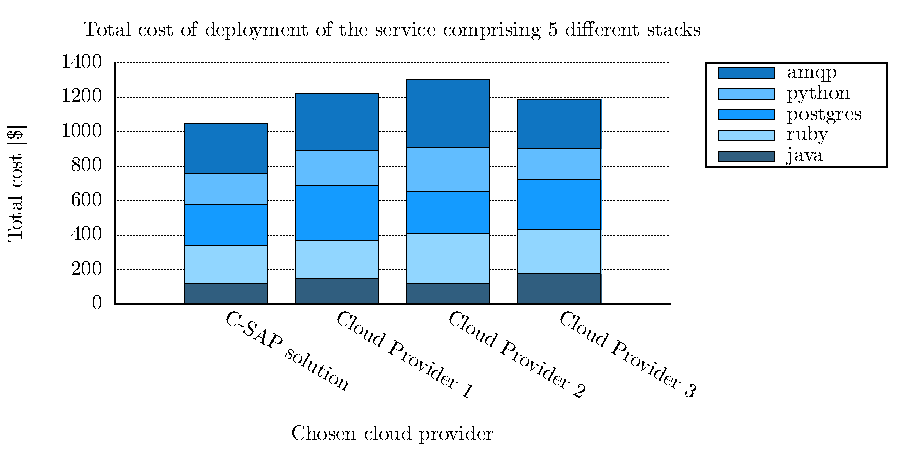
\includegraphics{chapter-7/case-study-service-deployment-reduced-client-costs}
  \end{center}
  \caption{Comparison of the deployment cost when the service is deployed only on a selected cloud provider or a combination of cloud providers selected by Cloud-SAP}
  \label{ch7:service-deployment-cost}
\end{figure}

\section{Auto-scaling}
